\chapter{Sphere collision}
\label{cha:spherecollision}

Spheres are the simplest of bounding shapes used in collision detection. This chapter presents tests for two versions of algorithms - naive $O(N^2)$ approach and with partitioned space. While simpler algorithm has far greater number of collision checks per frame, it allocates almost no memory per frame. More complex method will minimise number of checks, but additional structure and steps added may influence overall execution time in unexpected way.


\begin{figure}[h!]
  \caption{Example rendering of tested sphere collision system}
  \label{img:spheres}
  \centering
	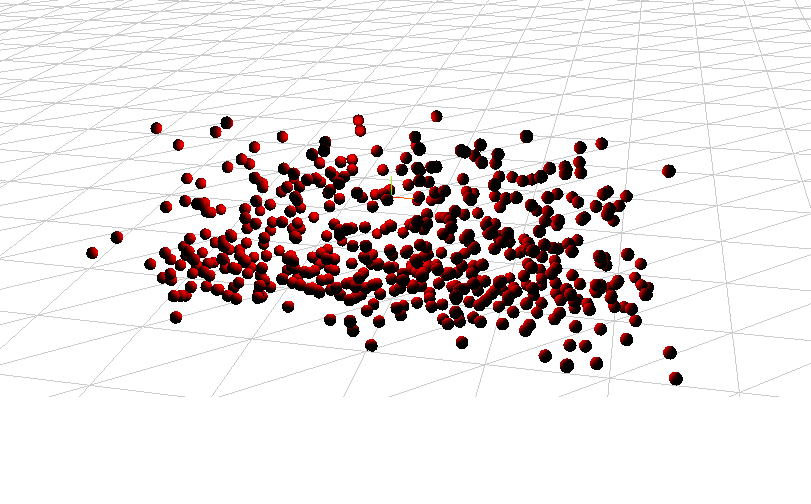
\includegraphics[width=16cm]{spheres/render.png}
\end{figure}

\section{Algorithm description}
\label{sec:spherealgorithmdescription}

Collision detection for spheres is a trivial task. If distance between two spheres is smaller than sum of their radiuses, spheres collide.

$\sqrt{(S_1.x - S_2.x)^2 + (S_1.y - S_2.y)^2 + (S_1.z - S_2.z)^2} < S_1.radius + S_2.radius$

While the equation is simple, with large number N of colliding objects complexity of this detection is $O(N^2)$. Methods of space partitioning are used to reduce number of checks. One used in this benchmark is Octree.
Base for algorithm is a tree-like structure of bounding boxes. Whenever a box contains more than one colliding object, it's divided into eight smaller boxes, by partitioning each edge by 2. When maximum tree depth is reached, multiple objects are stored in one box. One object may be referenced from multiple boxes, when it's size and position make them intersect. Each movement requires a check if object has already moved to one of neighbour boxes.

\begin{figure}[h!]
  \caption{Octree structure. Source: http://en.wikipedia.org/wiki/File:Octree2.svg/}
  \label{img:octree2}
  \centering
	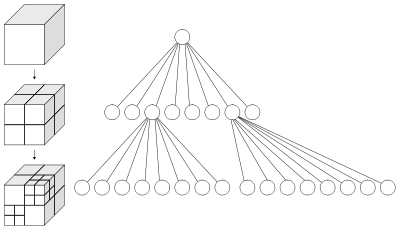
\includegraphics[width=10cm]{octree/octree2.png}
\end{figure} 

Having objects grouped in boxes reduces complexity of collision check. Since an object may collide only with objects in the same box, number of checks is much smaller. Overall complexity of Octree checks is $O(N log{N})$.
TODO: reference for complexity.

\begin{figure}[h!]
  \caption{Example of WebGL Octree debug rendering. Available online at http://pawlowski.it/octtree/}
  \label{img:octree}
  \centering
	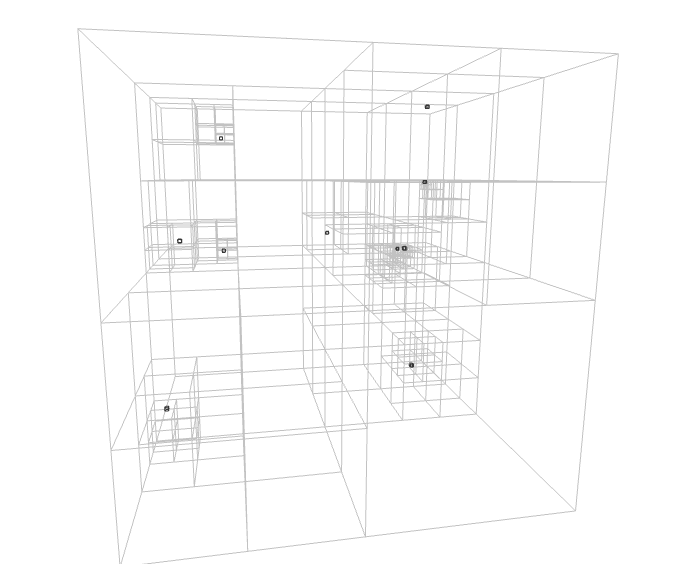
\includegraphics[width=10cm]{octree/octree.png}
\end{figure} 

When collision is detected, collision response is calculated. It's result is directly derived from rule of conservation of momentum and conservation of kinetic energy.

$m_1*\vec{v_1} + m_2*\vec{v_2} = m_1*\vec{v'_1} + m_2*\vec{v'_2}$

$\frac{m_1}{2}*\vec{v_1}^2 + \frac{m_2}{2}*\vec{v_2}^2 = \frac{m_1}{2}*\vec{v'_1}^2 + \frac{m_2}{2}*\vec{v'_2}^2$

TODO: add math here, finish this chapter.

\section{{$O(N^2)$} approach}
\label{sec:sphereinitial}

Naive approach for collision detection proves to by easy to implement in JavaScript. Since almost no memory is allocated in each frame, no garbage collection issues appear. All methods are well defined and work mostly on floats. This results in highly optimised binary code produced by compiler, as show on \ref{img:spheres1profile}.

\begin{figure}[h!]
  \caption{Chart of time used in optimised version of JavaScript}
  \label{img:spheres1profile}
  \centering
	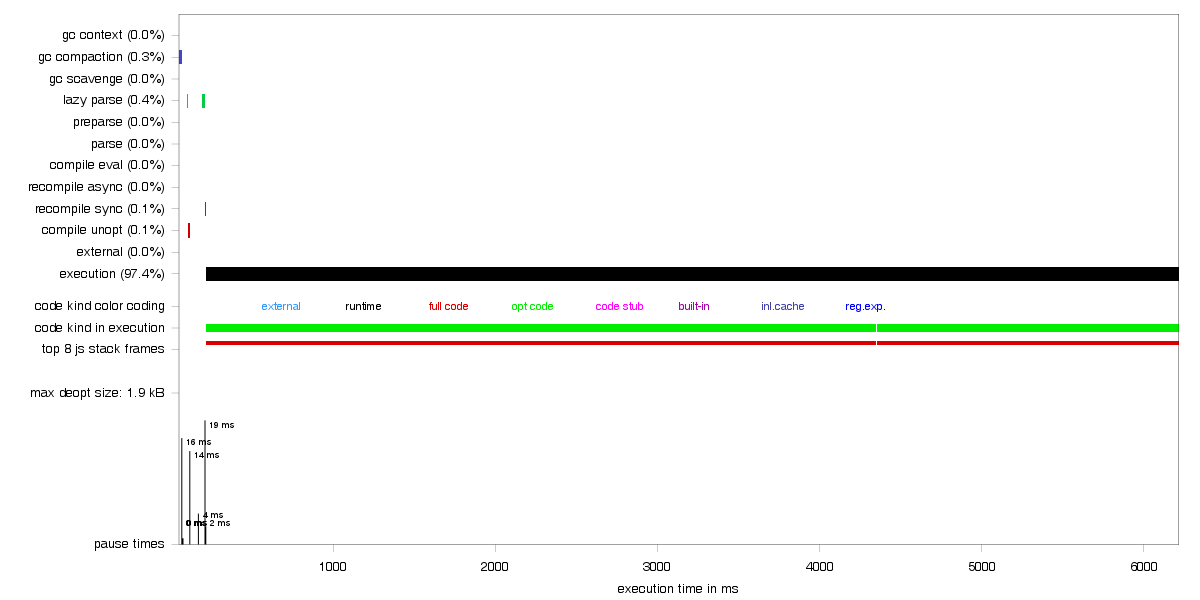
\includegraphics[width=16cm]{spheres/spheres1-profile.png}
\end{figure} 

Multiple tests with N=1000 and different number of frames rendered show, that for simple mathematical task performance of JavaScript is very close to those of C++. On average, JavaScript version of benchmark runs 15\% longer than C++ one.

\begin{figure}[h!]
  \caption{Comparison of total execution time. N = 1000, varying number of frames.}
  \label{img:spheres1-time-total}
  \centering
	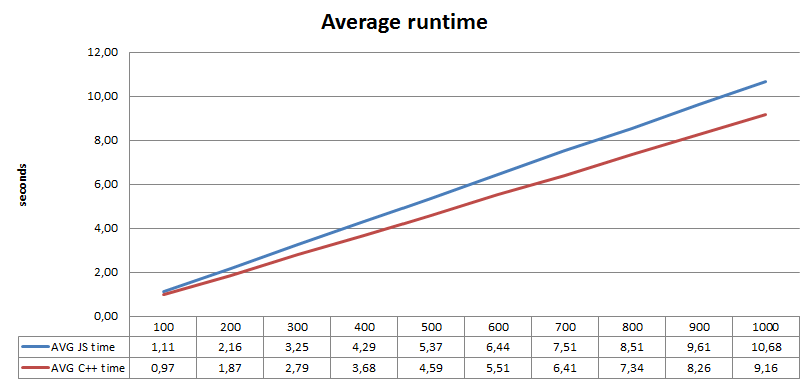
\includegraphics[width=16cm]{spheres/time-total.png}
\end{figure} 


\begin{figure}[h!]
  \caption{Comparison of execution time per frame. N = 1000, varying number of frames.}
  \label{img:spheres1-time-per-frame}
  \centering
	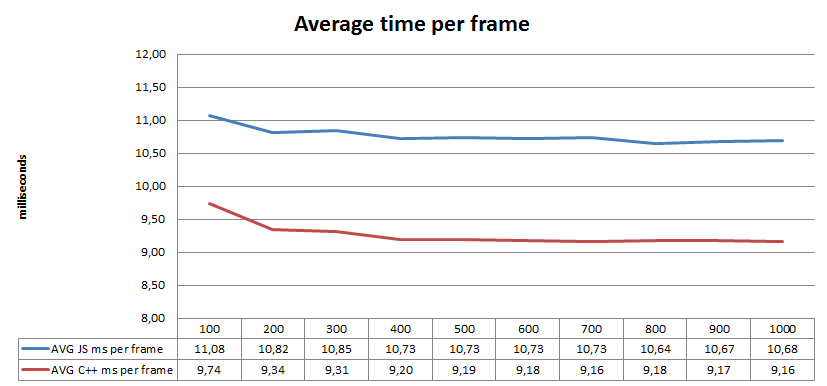
\includegraphics[width=16cm]{spheres/time-per-frame.png}
\end{figure} 


\section{Octree-partitioned space}
\label{sec:sphereoctree}
